\chapter{Proposta e Plano de Continuidade}

Neste capítulo é apresentada a proposta deste trabalho, com os requisitos, estórias de usuário, casos de uso e demais artefatos
que fazem parte do levantamento de requisitos e análise, oferecendo uma visão ampla da aplicação que será desenvolvida.
Além disso, também é apresentado o plano de continuidade com o cronograma para realização das etapas da segunda parte deste
trabalho.

Para o desenvolvimento completo desse projeto é previsto a realização de 4 etapas, ao longo dos meses referentes ao segundo
período letivo de 2021 da Universidade Federal de Sergipe (UFS), estas são listadas a seguir:
\begin{itemize}
    \item Desenvolvimento do aplicativo com a implementação dos requisitos mais essenciais e viáveis;
    \item Revisão e testes da acessibilidade da aplicação;
    \item Descrição do processo metodológico e análise dos resultados;
    \item Revisão, correção e entrega do trabalho.
\end{itemize}

Este projeto está sendo desenvolvido em parceria com a mestranda, Débora Almeida Silveira Sobral, do
Programa de Pós-graduação Profissional em Gestão e Inovação Tecnológica em Saúde (PPGITS), também orientanda da Profa.
Dra. Adicinéia Aparecida de Oliveira. E tem como objetivo
o desenvolvimento de uma aplicação móvel como ferramenta de auxilio à educação e ao autocuidado de pacientes diabéticos
com acuidade visual prejudica, acessível à PDV\@.

Para tanto, em \citeonline{Sobral2021} foi realizado um levantamento de referencial teórico e tecnológico sobre o DM,
aplicativos móveis e deficiência visual. Assim, reunindo as principais funcionalidades e soluções que o aplicativo a ser
desenvolvido deveria adotar como requisitos para que atendesse às necessidades desse público-alvo.

\newpage

\section{Busca de Anterioridade}

Em \citeonline{Sobral2021}, realizou-se uma busca de anterioridade, na base do Instituto Nacional de Propriedade Industrial (INPI)
e nas lojas de aplicativos Google Play (Android) e Apple Store (iOS), visando identificar os \emph{softwares} e funcionalidades
já existentes sobre DM e DV no mercado.

A \autoref{fig_tab_cor_func} exibe uma tabela onde a autora buscou relacionar os \emph{apps} encontrados
nas lojas de aplicativos às principais funcionalidades propostas em seu trabalho para o DiaVision.

\begin{figure}[htb]
    \caption{\label{fig_tab_cor_func}Relação de funcionalidades dos \emph{apps} encontrados nas lojas de aplicativos.}
    \begin{center}
        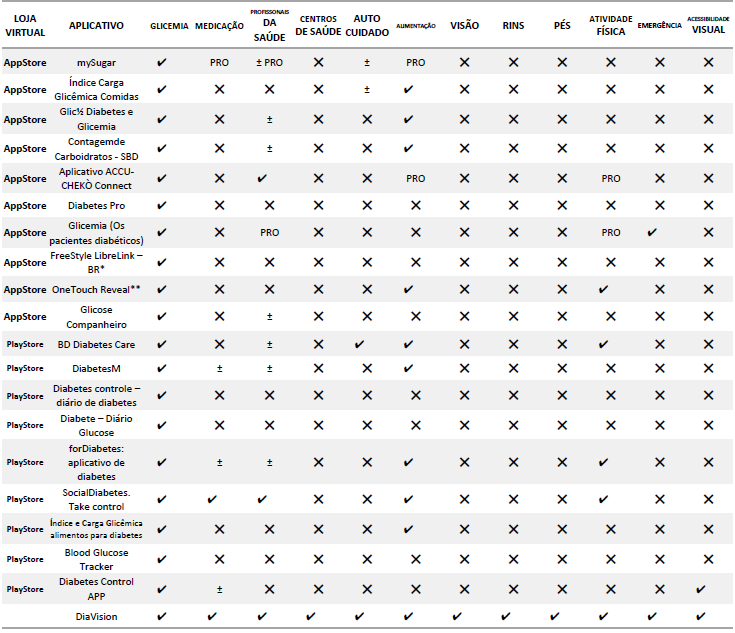
\includegraphics[scale=0.8]{Imagens/proposta/busca_anterioridade.png}
    \end{center}
    \legend{Fonte: \cite{Sobral2021}.}
\end{figure}

\newpage

\section{Visão e Análise}

Nesta seção são descritas as necessidades e características esperadas do produto de \emph{software} a ser desenvolvido, identificadas a partir de
reuniões com a \emph{product owner} (dona do produto), esta que identificou a problemática abordada neste trabalho e
realizou o levantamento de funcionalidades e problemas das soluções já existentes no mercado em \citeonline{Sobral2021}.

\subsection{Problema}

O problema que o produto busca resolver ficou definido como: a dificuldade de acesso à informações de autocuidado com relação
ao DM por deficientes visuais.

\subsection{Objetivo}

O objetivo do produto é fornecer, por meio de uma aplicação móvel, conteúdos e funcionalidades que auxiliem os diabéticos portadores de deficiências
visuais no gerenciamento do autocuidado com o DM\@.

\subsection{Diferenciais}

A acessibilidade ao deficiente visual é o principal diferencial do produto, como pode ser visto na \autoref{fig_tab_cor_func},
onde apenas um \emph{app} demonstrou possuir essa característica.

\subsection{Riscos e Impedimentos}

Os seguintes riscos e possíveis impedimentos com relação ao produto foram identificados:

\begin{itemize}
    \item Não adesão por parte do público alvo;
    \item Dificuldades no manuseio do \emph{smartphone} pelo público alvo;
    \item Dificuldade de localizar os possíveis participantes da pesquisa;
    \item Utilização incorreta do aplicativo ou não assimilação das informações adquiridas;
    \item Afastamento do paciente da assistência continuada na rede primária;
    \item Constrangimento do usuário por falta de entendimento das funcionalidades.
\end{itemize}

\newpage

\subsection{Estórias dos usuários}

No processo de definição e levantamento de requisitos, foram identificadas
as estórias dos usuários que são listadas na \autoref{tab-est-usr}.

\begin{table}[htb]
    \begin{center}
        \ABNTEXfontereduzida
        \caption{Relação de estórias dos usuários.}
        \label{tab-est-usr}
        \begin{tabular}{p{2.0cm}|p{5.0cm}|p{7.0cm}}
            %\hline
            \textbf{Eu, enquanto}                                          & \textbf{Quero} & \textbf{Para}                     \\
            \hline
            Paciente                                                       &
            Encontrar o \emph{app} nas lojas virtuais                      &
            Baixar o \emph{app} no meu celular.                                                                                 \\
            \hline
            Paciente                                                       &
            Realizar cadastro no aplicativo                                &
            Ter acesso às funcionalidades do \emph{app}.                                                                        \\
            \hline
            Paciente                                                       &
            Realizar login de forma prática                                &
            Para acessar as funcionalidades do \emph{app}.                                                                      \\
            \hline
            Paciente                                                       &
            Poder alterar minha senha                                      &
            Poder alterá\@-la e recuperar acesso ao \emph{app}.                                                                 \\
            \hline
            Paciente                                                       &
            Registrar informações das refeições                            &
            Acompanhar a quantidade de calorias consumidas por refeição.                                                        \\
            \hline
            Paciente                                                       &
            Ter acesso a aplicativos acessíveis para deficientes visuais   &
            Ajudar a realizar atividades do dia a dia.                                                                          \\
            \hline
            Paciente                                                       &
            Sugerir aplicativos acessíveis para deficientes visuais        &
            Compartilhar aplicativos que possam ajudar outros usuários com DV\@.                                                \\
            \hline
            Paciente                                                       &
            Registrar práticas de atividade física                         &
            Acompanhar a evolução da rotina de atividade física.                                                                \\
            \hline
            Paciente                                                       &
            Ter acesso à dicas de autocuidado                              &
            Melhorar a qualidade de vida e prevenir complicações do DM\@.                                                       \\
            \hline
            Paciente                                                       &
            Filtrar as dicas por categorias                                &
            Facilitar a busca das dicas sobre assuntos específicos.                                                             \\
            \hline
            Paciente                                                       &
            Consultar locais para acesso à serviços de saúde               &
            Facilitar o acesso e contato com as principais clínicas, hospitais e consultórios da cidade.                        \\
            \hline
            Paciente                                                       &
            Registrar glicemia                                             &
            Acompanhamento dos valores de glicemia e ser alertado quando estiver fora do limite.                                \\
            \hline
            Paciente                                                       &
            Registrar medicações que faço uso                              &
            Ter uma lista atualizada com todas as informações das medicações e ser alertado dos horários de uso das medicações. \\
            \hline
            Paciente                                                       &
            Realizar avaliação dos pés                                     &
            Acompanhar a evolução dos pés e detectar quando surgir alterações.                                                  \\
            \hline
            Paciente                                                       &
            Registrar diurese diária                                       &
            Acompanhar quando surgir alterações.                                                                                \\
            \hline
            Paciente                                                       &
            Ter acesso a relatórios dos dados registrados                  &
            Visualizar e compartilhar esses dados registrados.                                                                  \\
            \hline
            Paciente                                                       &
            Ter acesso aos dados pessoais                                  &
            Editar ou acrescentar dados pessoais durante o uso do aplicativo.                                                   \\
            \hline
            Paciente                                                       &
            Configurar notificações                                        &
            Definir horários e quais ativar ou desativar.                                                                       \\
            \hline
            Paciente                                                       &
            Configurar preferências                                        &
            Personalizar os limites da glicemia.                                                                                \\
            \hline
            Paciente                                                       &
            Realizar \emph{logout}                                         &
            Para desvincular minha conta do \emph{app}.                                                                         \\
            \hline
            Administrador do sistema                                       &
            Adicionar dicas de autocuidado para os pacientes               &
            Fornecer informações acerca de cuidados com a saúde.                                                                \\
            \hline
            Administrador do sistema                                       &
            Cadastrar centros de saúde no sistema                          &
            Que o paciente possa conhecer os centros de saúde que atendem suas demandas.                                        \\
            \hline
            Administrador do sistema                                       &
            Cadastrar sugestões de aplicativos acessíveis no sistema       &
            Que o paciente possa conhecer outros \emph{apps} acessíveis que possam ajudá\@-lo no cotiano.                       \\
            \hline
            Administrador do sistema                                       &
            Aprovar/recusar as sugestões de centros de saúde e aplicativos &
            Assegurar credibilidade ao aplicativo.                                                                              \\
            % \hline
        \end{tabular}
        \legend{Fonte: Autores.}
    \end{center}
\end{table}

\newpage

\subsection{Casos de Uso}

A partir dos requisitos e estórias dos usuários identificados, o diagrama de casos de usos da \autoref{fig_use_cas} foi elaborado.

\begin{figure}[htb]
    \caption{\label{fig_use_cas}Diagrama de casos de uso.}
    \begin{center}
        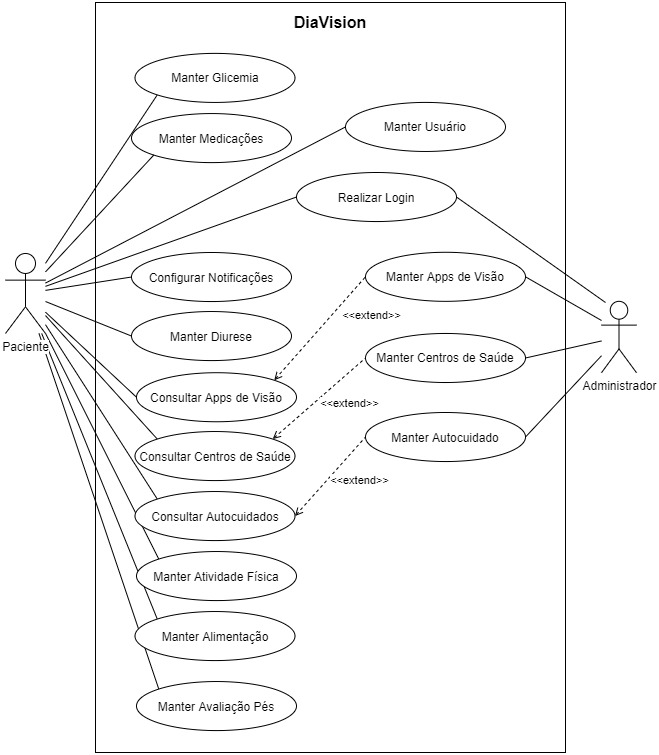
\includegraphics[scale=0.65]{Imagens/proposta/use_case.jpg}
    \end{center}
    \legend{Fonte: Autor.}
\end{figure}

\newpage

\section{Cronograma}

Por fim, o cronograma na \autoref{fig_cro_con} foi definido visando a organização e planejamento das atividades que serão realizadas
na segunda parte desse trabalho.

\begin{figure}[htb]
    \caption{\label{fig_cro_con}Cronograma de continuidade do Projeto.}
    \begin{center}
        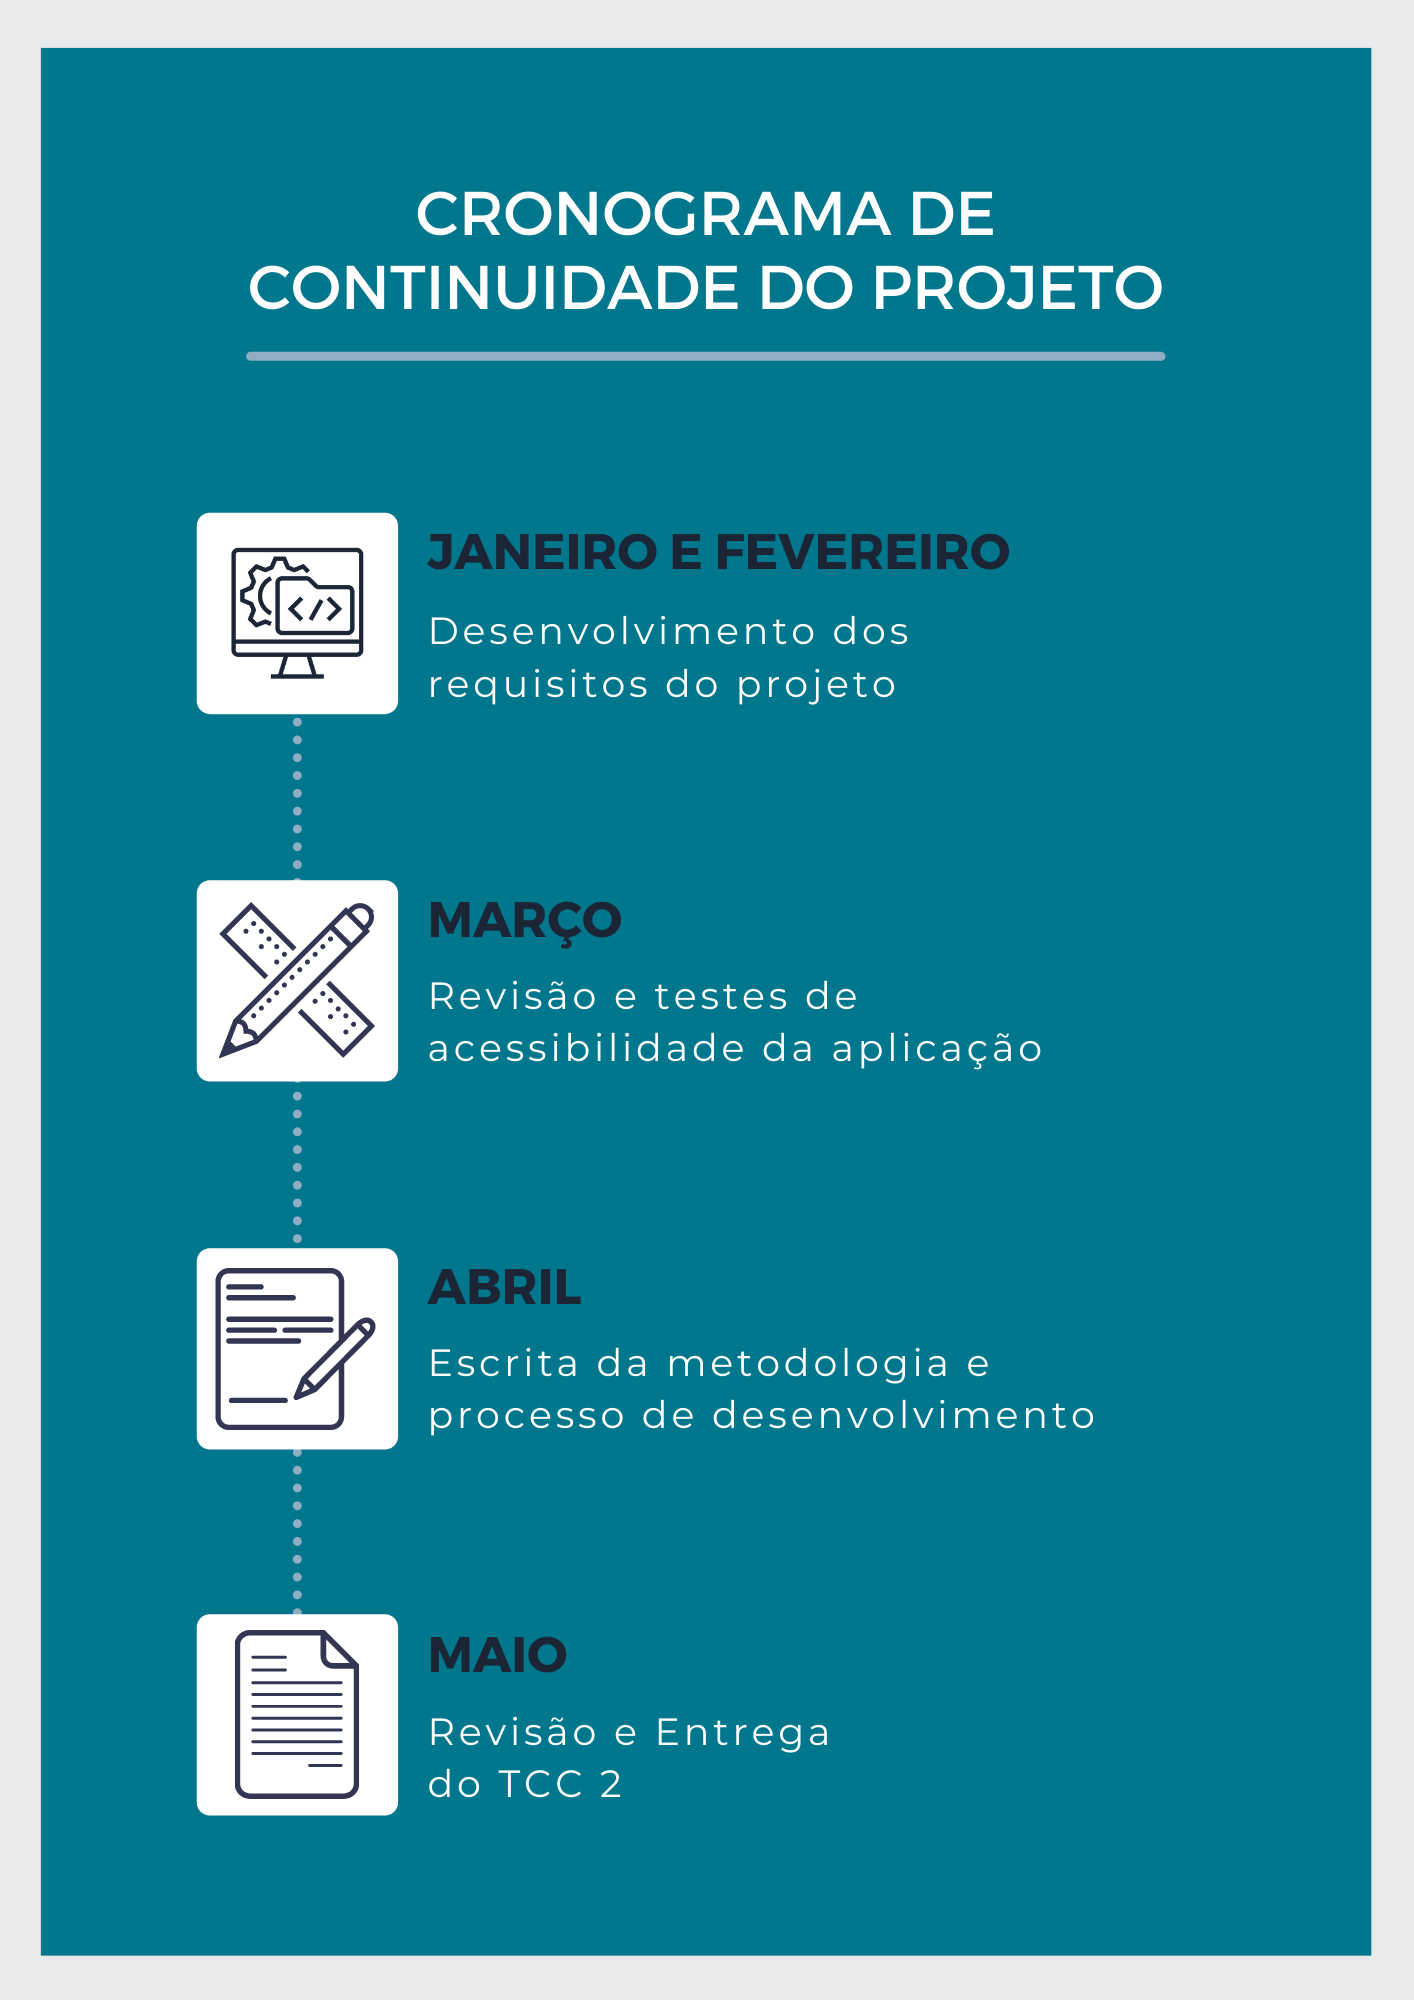
\includegraphics[scale=0.65]{Imagens/proposta/cronograma_continuidade.png}
    \end{center}
    \legend{Fonte: Autor.}
\end{figure}